\documentclass{beamer}

\usepackage{fontspec}
\usepackage{float}

%\setmainfont{STSong}
\setmainfont{STHeitiSC-Light}
%\setmainfont{Hei}

%\setsansfont{STSong}            % Set Title font
\setsansfont{Hei}            % Set Title font

\setmonofont{STSong}

\usetheme{metropolis}           % Use metropolis theme

\usepackage{graphicx}

\title{人工智能的哲学思考}
\date{2018 3/12} 
\author{葛天逸,陈东箭,李陈豪,戚伏波,王韧,张思钧}
\institute{马克思主义基本原理概论课堂讨论} 
\begin{document}
  \maketitle
  \tableofcontents

  \section{人工智能的定义}
  \begin{frame}{人工智能的定义}
    人工智能    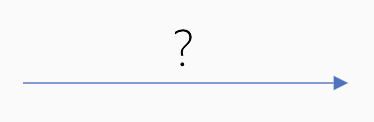
\includegraphics[width=1in]{qfbPic1} 技术奇点

   \begin{figure}[H]
   \centering
    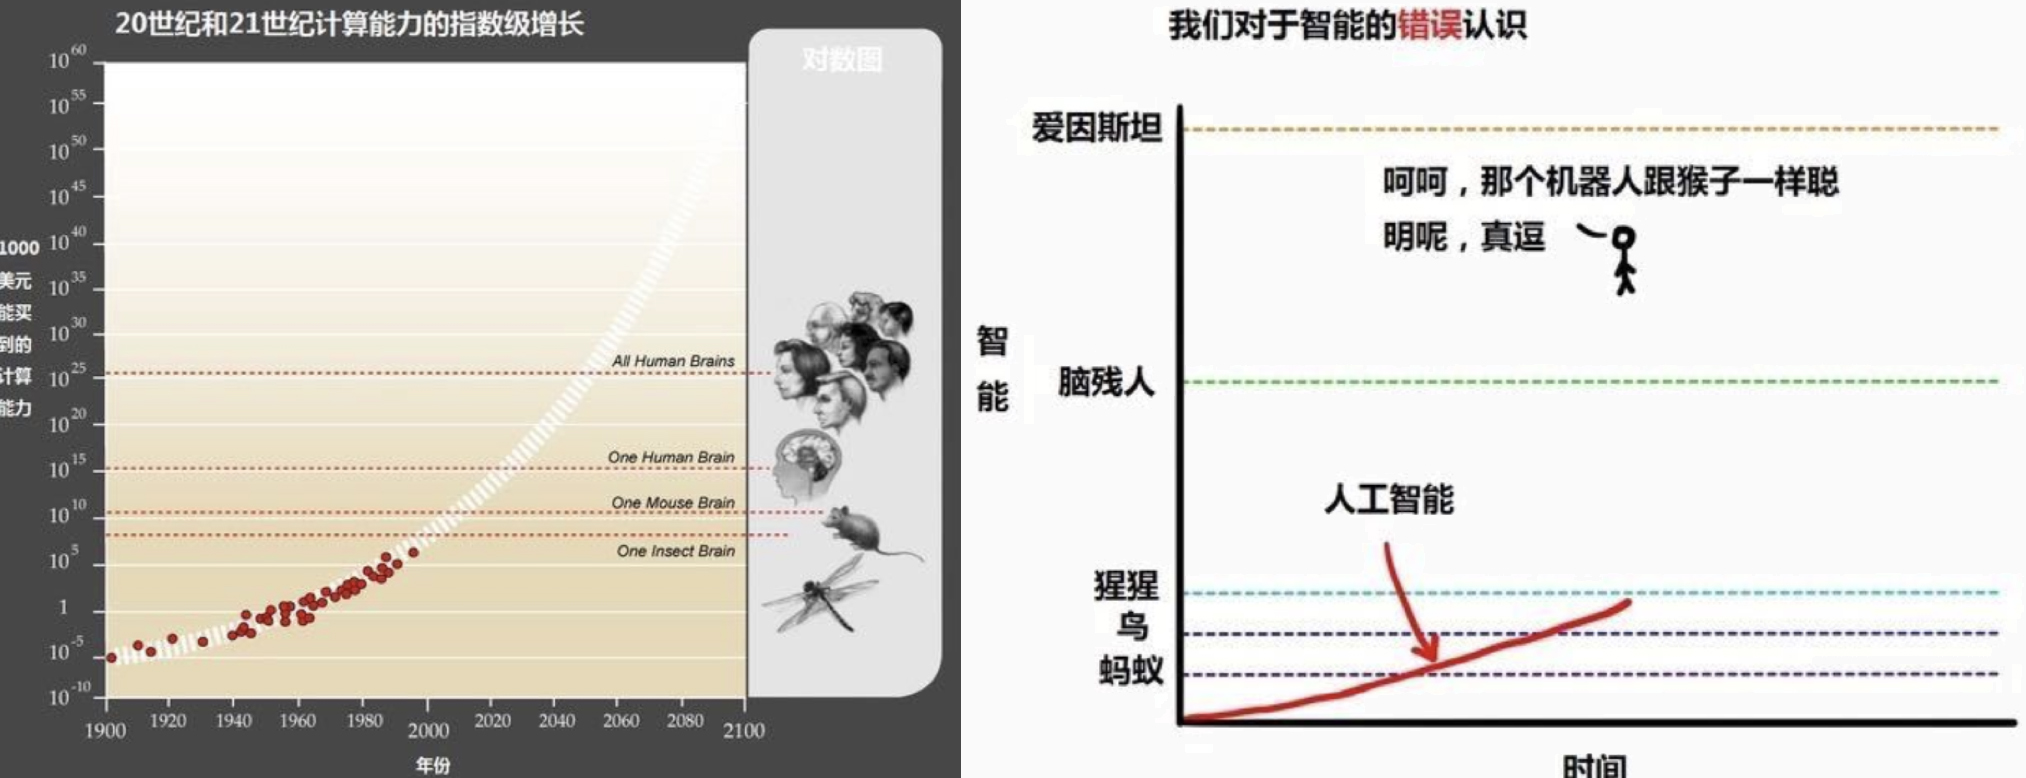
\includegraphics[width=4.5in]{qfbPic2.jpg}
   \end{figure}

  \end{frame}

  \begin{frame}{人工智能的定义}
     \begin{figure}[H]
   \centering
    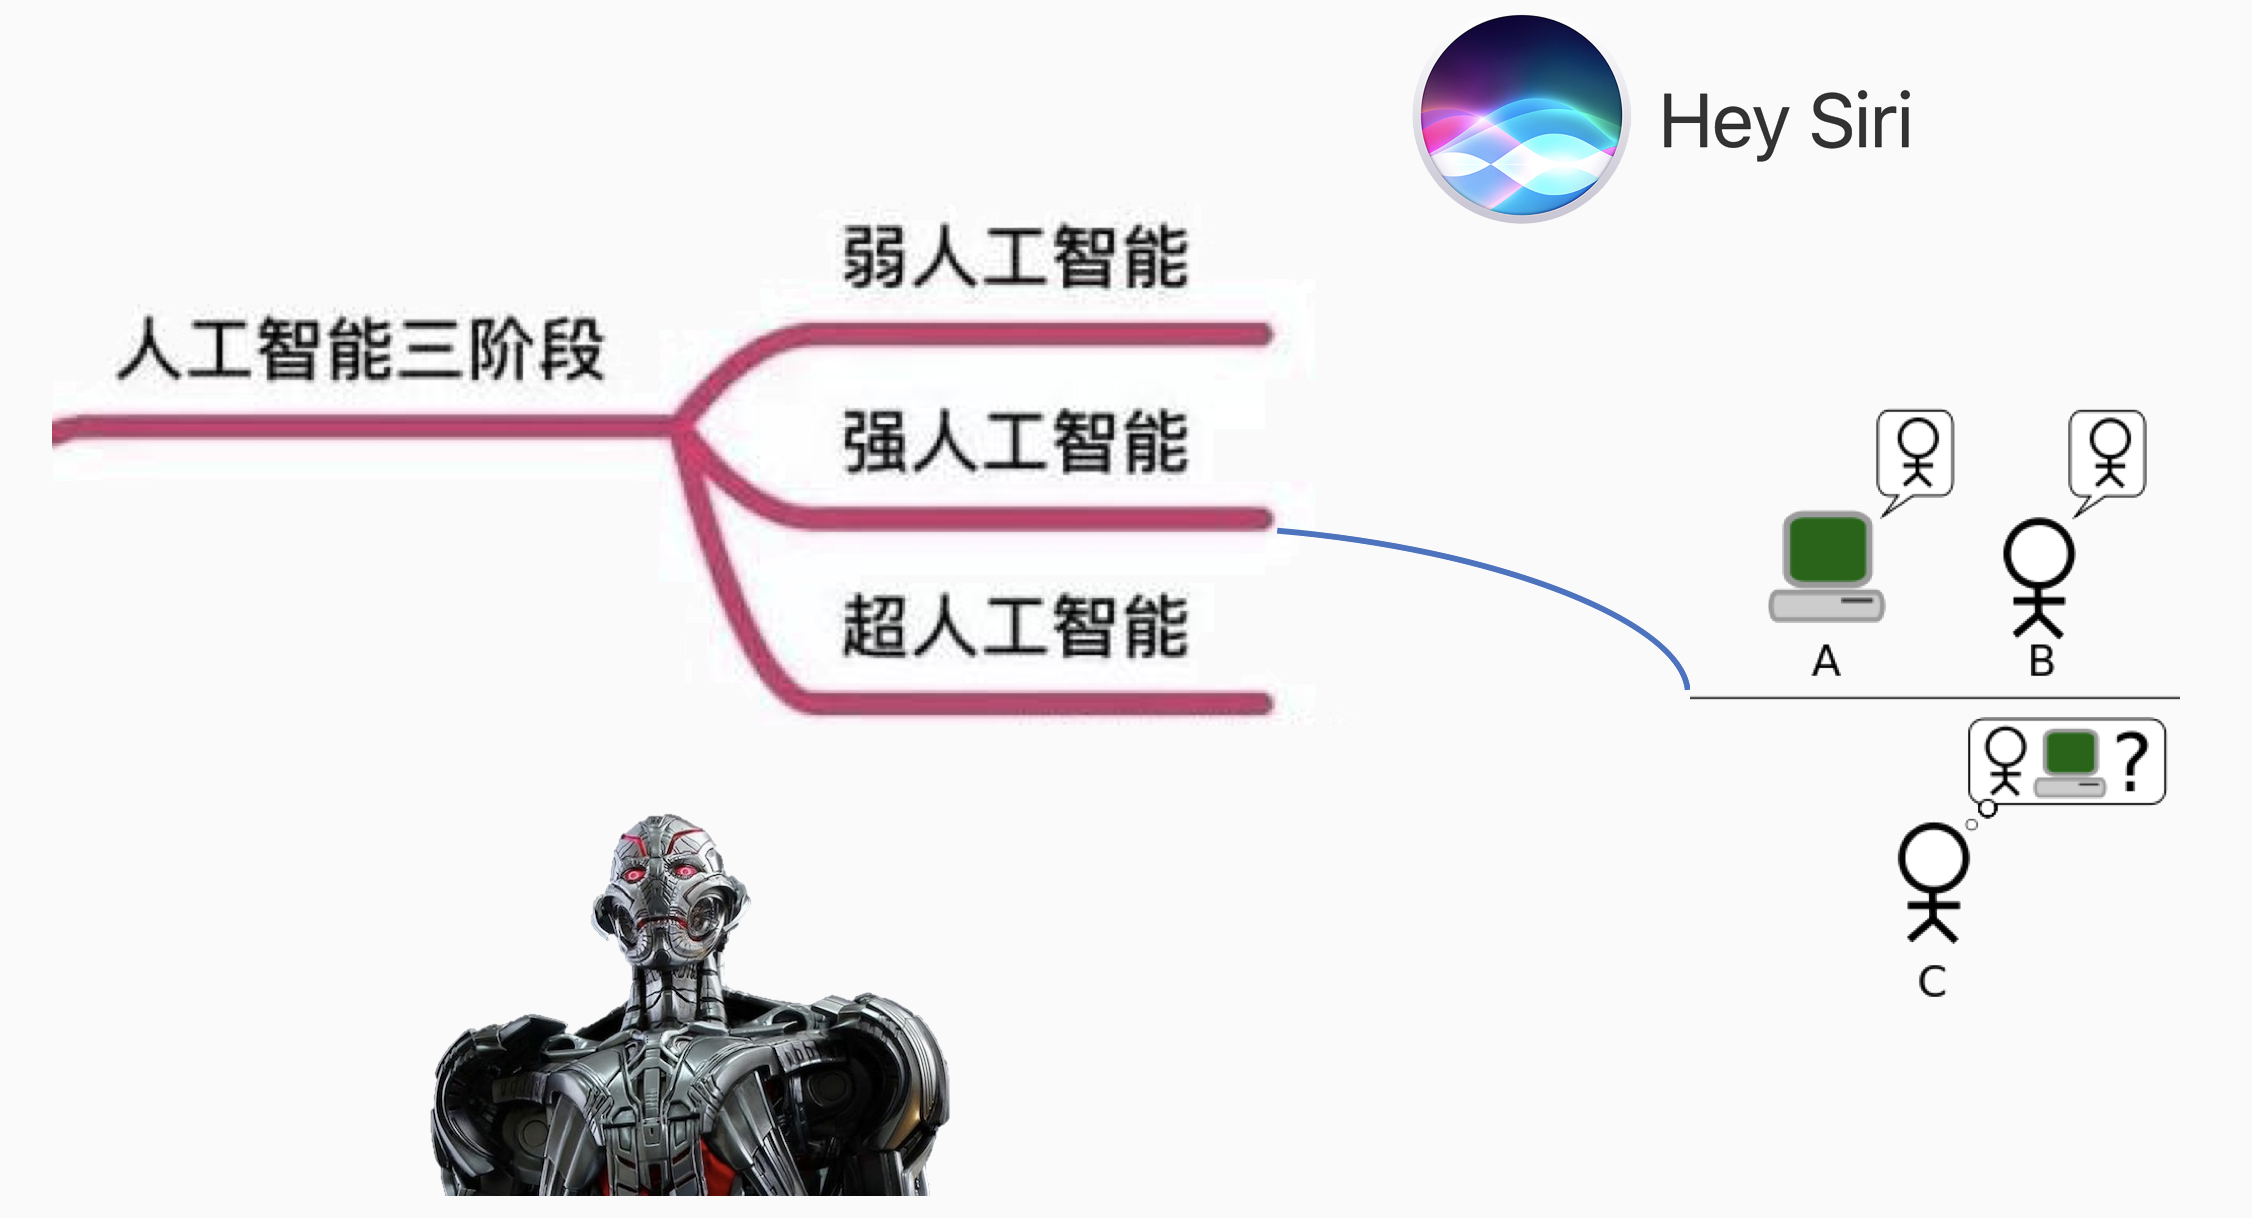
\includegraphics[width=4.5in]{qfbPic3.jpg}
   \end{figure}
  \end{frame}

  \section{人与人工智能关系的猜想}
  \begin{frame}{人与人工智能关系的猜想}
    \begin{itemize}
     \item 融合改造
     \item 共同生活
     \item 权限控制
    \end{itemize}
  \end{frame}

  \begin{frame}{人与人工智能关系的猜想}
    \begin{itemize}
     \item  人与人工智能融合改造
    \end{itemize}
   \begin{figure}[H]
   \centering
   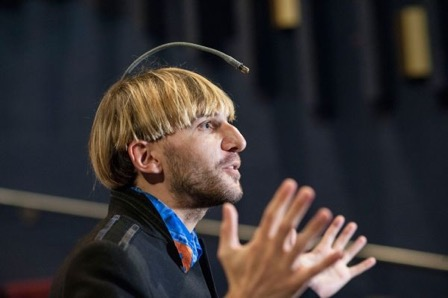
\includegraphics[width=2.5in]{gtyPic1.jpg}
   \end{figure}
  \end{frame}

  \begin{frame}{人与人工智能融合改造}
  \begin{quote}
    \hspace*{0.21in} 人的本质不是单个人所固有的抽象物,在其现实性上,\\
    他是一切社会关系的总和”
    \begin{flushright}
    ——马克思《关于费尔巴哈的提纲》
    \end{flushright}
  \end{quote}
  \end{frame}

 \begin{frame}{人与人工智能关系的猜想}
    \begin{itemize}
     \item  人对人工智能有最高权限
    \end{itemize}

   \begin{figure}[H]
   \centering
   
\includegraphics[width=4.3in]{gtyPic2.jpg}
   \end{figure}

  \end{frame}

 \begin{frame}{人对人工智能有最高权限}
    \begin{itemize}
     \item  阻止意识的能动作用?
    \end{itemize}

   \begin{figure}[H]
   \centering
   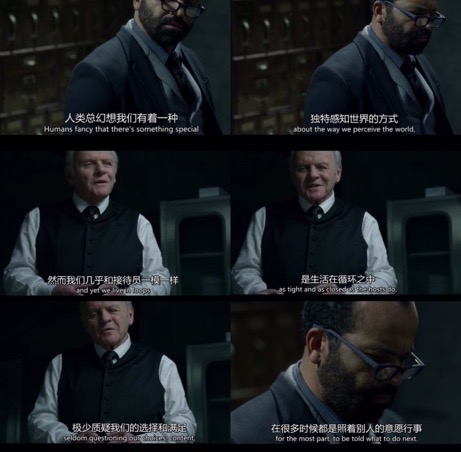
\includegraphics[width=4.25in]{gtyPic3.jpg}
   \end{figure}

  \end{frame}

\section{人工智能技术的社会问题}
  \begin{frame}{人工智能技术的社会问题}
   \begin{figure}[H]
   \centering
   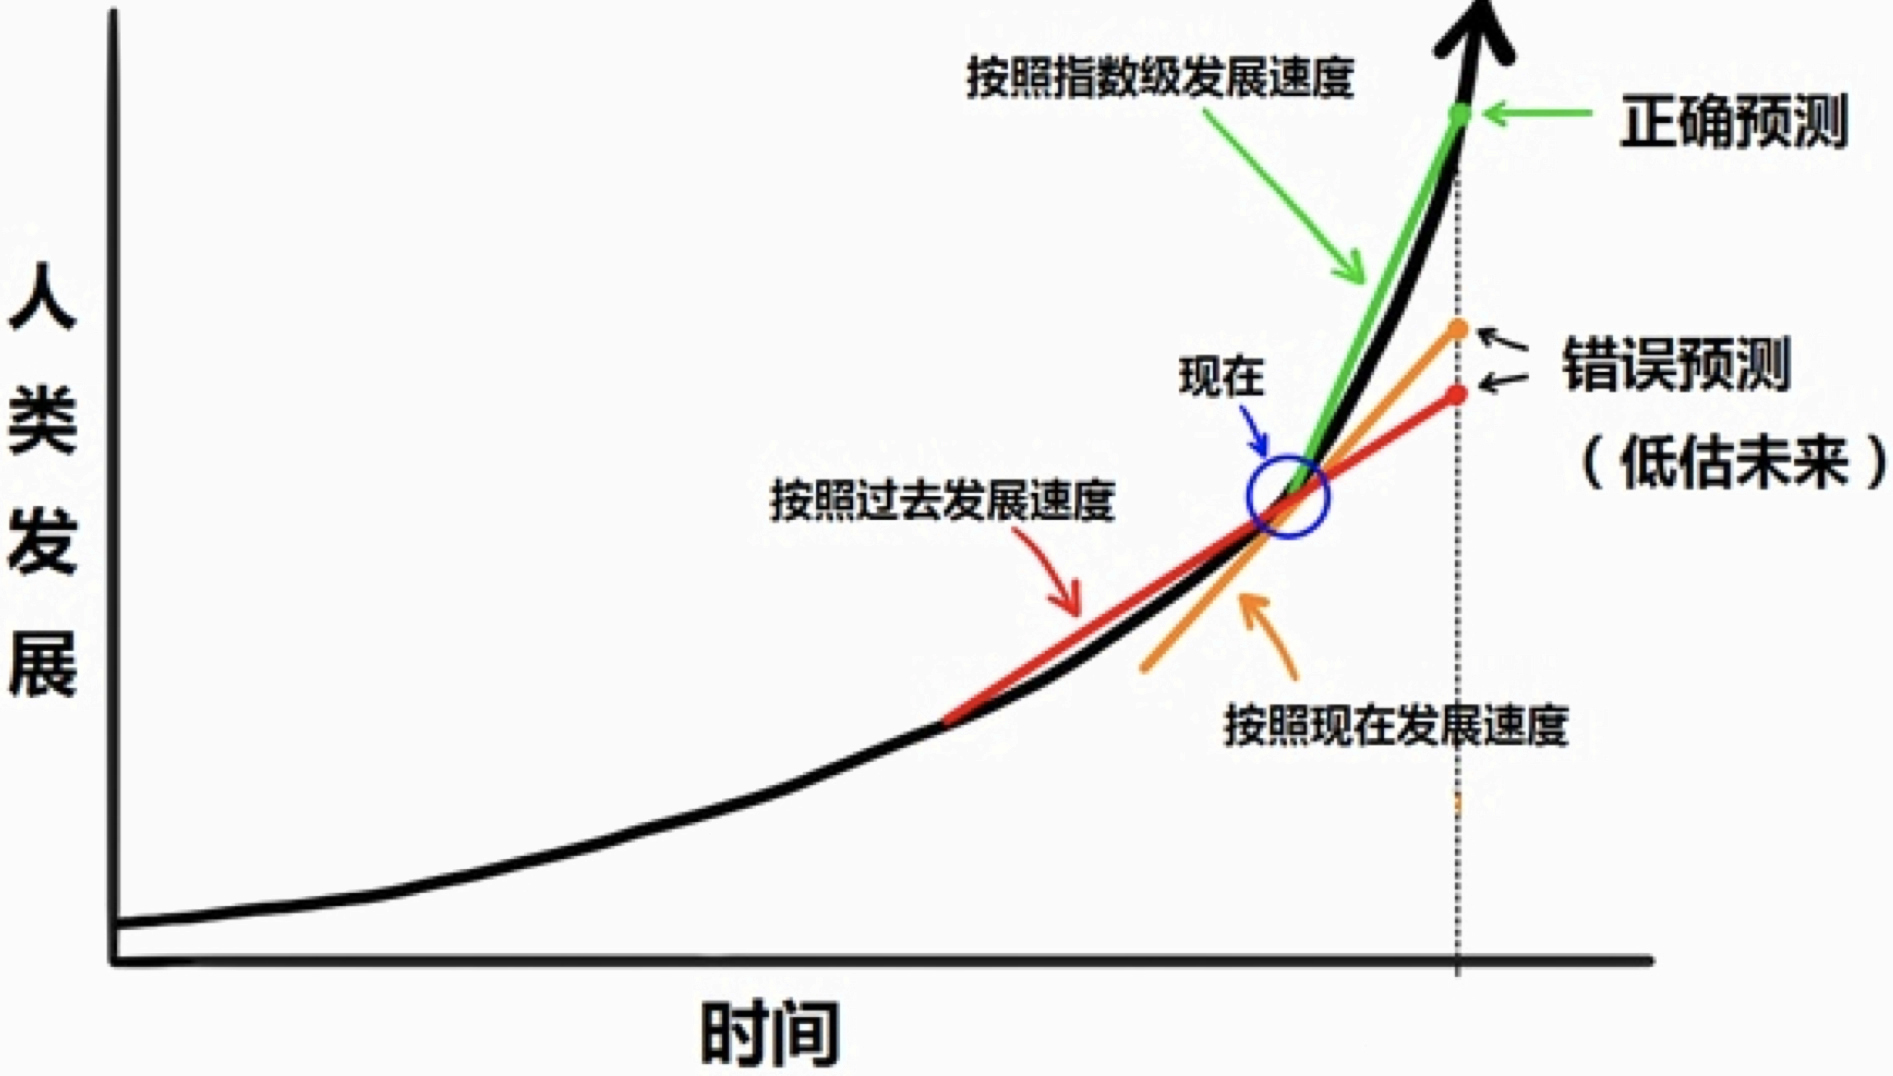
\includegraphics[height=2.5in]{zsjPic1.jpg}
   \end{figure}
  \end{frame} 

\begin{frame}{人工智能技术的社会问题}
  \begin{itemize}
   \item 不确定性
  \end{itemize}

  \begin{figure}[H]
   \centering
   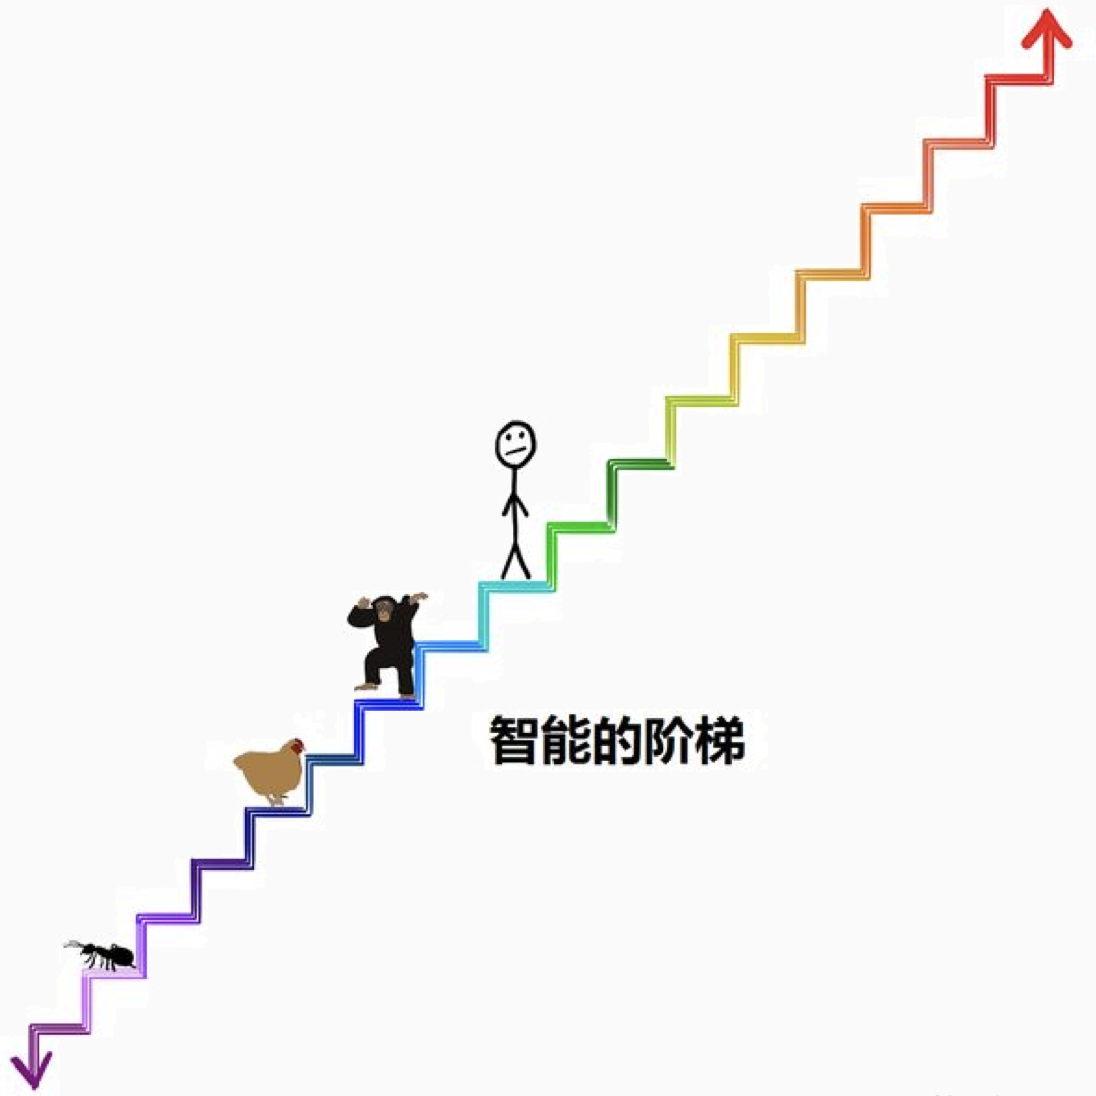
\includegraphics[width=1.9in]{zsjPic2.jpg}
   \hspace*{0.3in}
   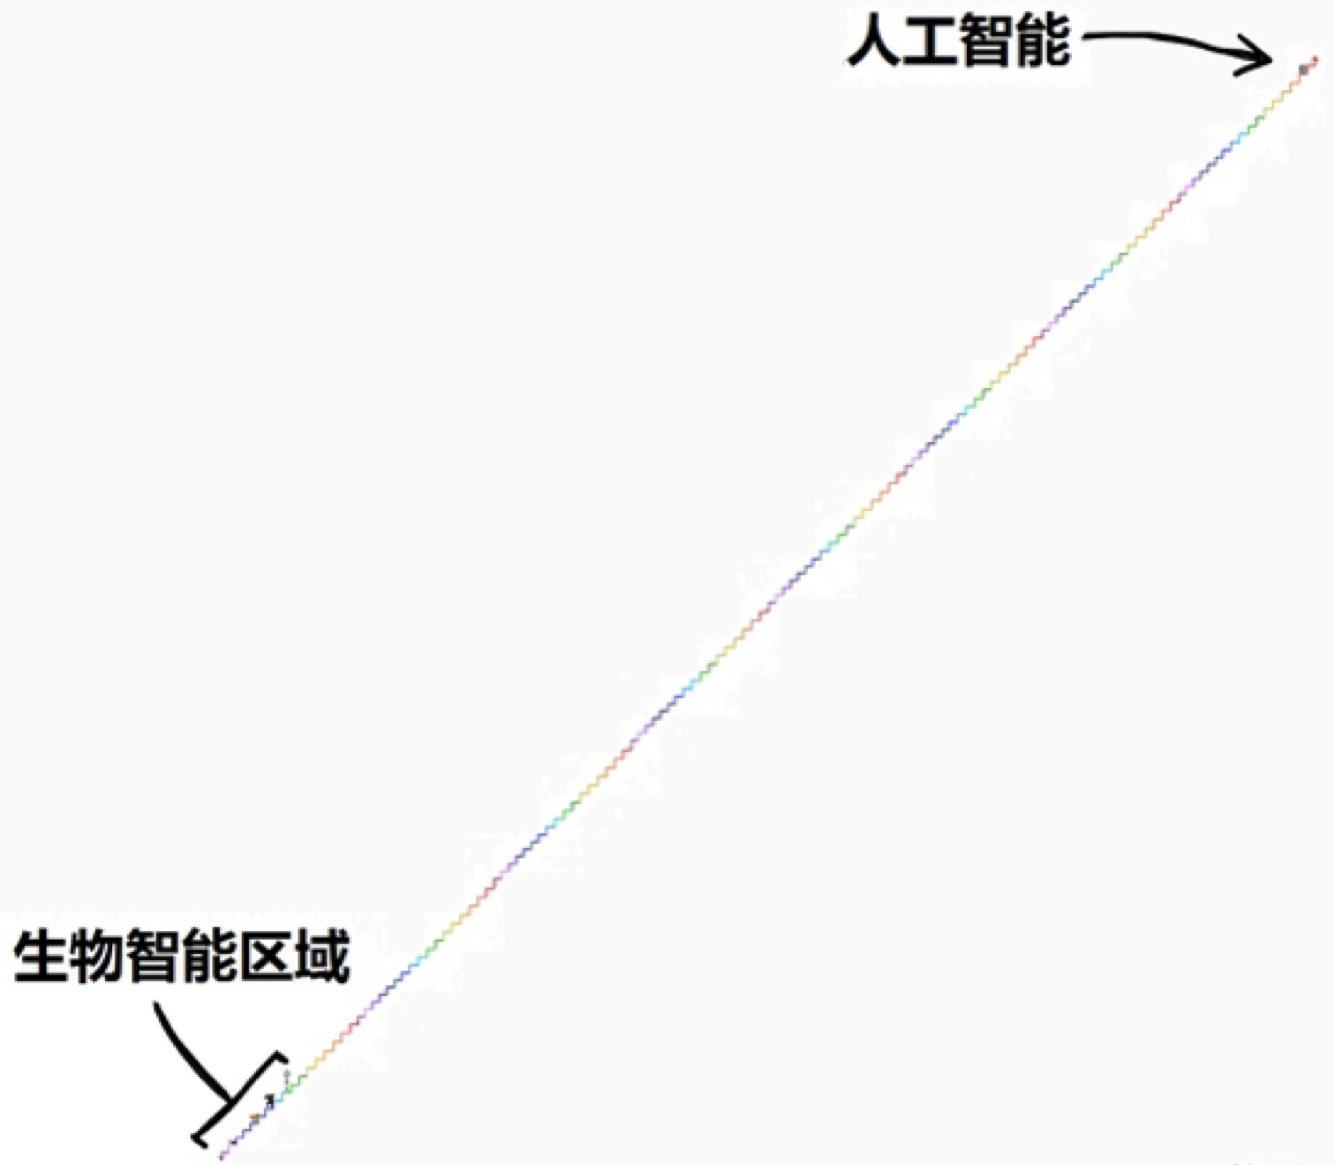
\includegraphics[width=1.9in]{zsjPic3.jpg}
   \end{figure}

\end{frame} 

\begin{frame}{人工智能技术的社会问题}
  \begin{itemize}
    \item 伦理问题 
      \begin{itemize}
       \item  环境伦理问题 
      \end{itemize}
  \end{itemize}

  \begin{figure}[H]
   \centering
   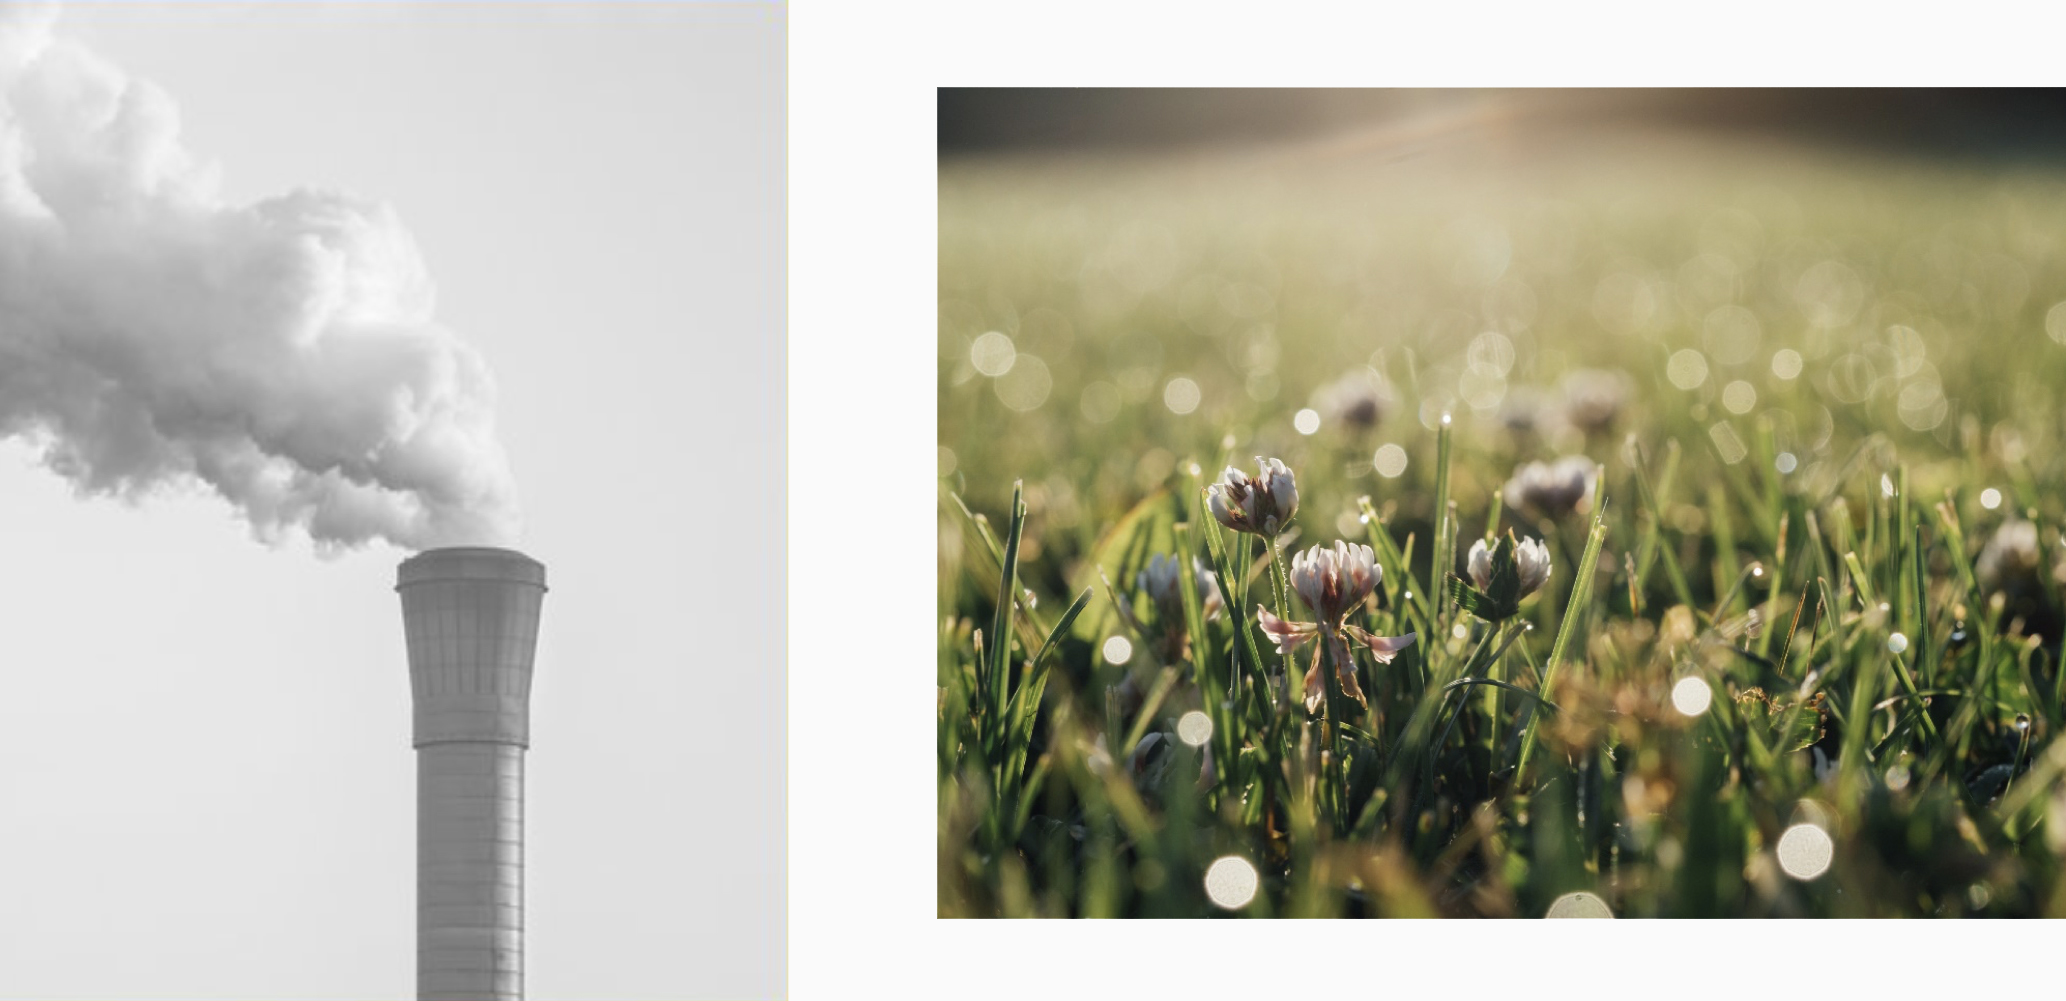
\includegraphics[width=4.3in]{zsjPic4.jpg}
   \end{figure}
  \end{frame}

\begin{frame}{人工智能技术的社会问题}
  \begin{itemize}
    \item 伦理问题 
      \begin{itemize}
       \item  环境伦理问题 
       \item  赋予道德地位
      \end{itemize}
  \end{itemize}

  \begin{figure}[H]
   \centering
   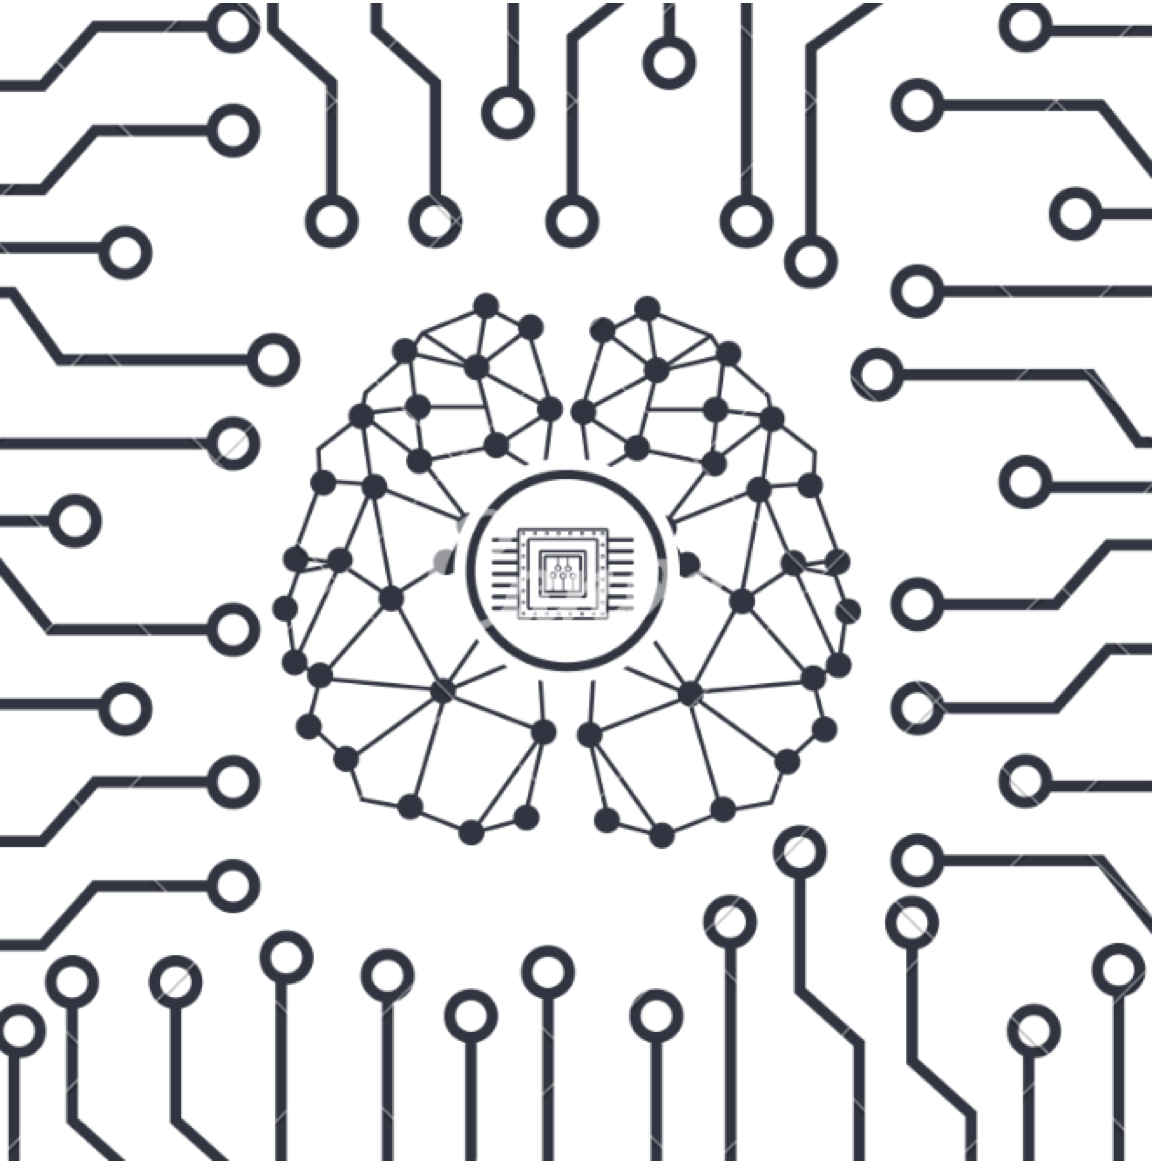
\includegraphics[height=1.7in]{zsjPic5.jpg}
   \end{figure}

\end{frame} 

  \section{人工智能的人权问题}
  \begin{frame}{人工智能的人权问题}
    \begin{itemize}
     \item 人权:人因其为人而应享有的权利
     \item 人工智能脱胎于人类文化
     \item 「人权」的概念服务于人类自身  
     \item 如果人工智能可融入人类,那么「意识」为何
    \end{itemize}
  \end{frame}

  \section{人工智能未来发展}

  \begin{frame}{人工智能未来发展}
    \begin{itemize}
     \item  如果未来机器拥有了人性,人类该如何自处?
    \end{itemize}
   \begin{figure}[H]
   \centering
   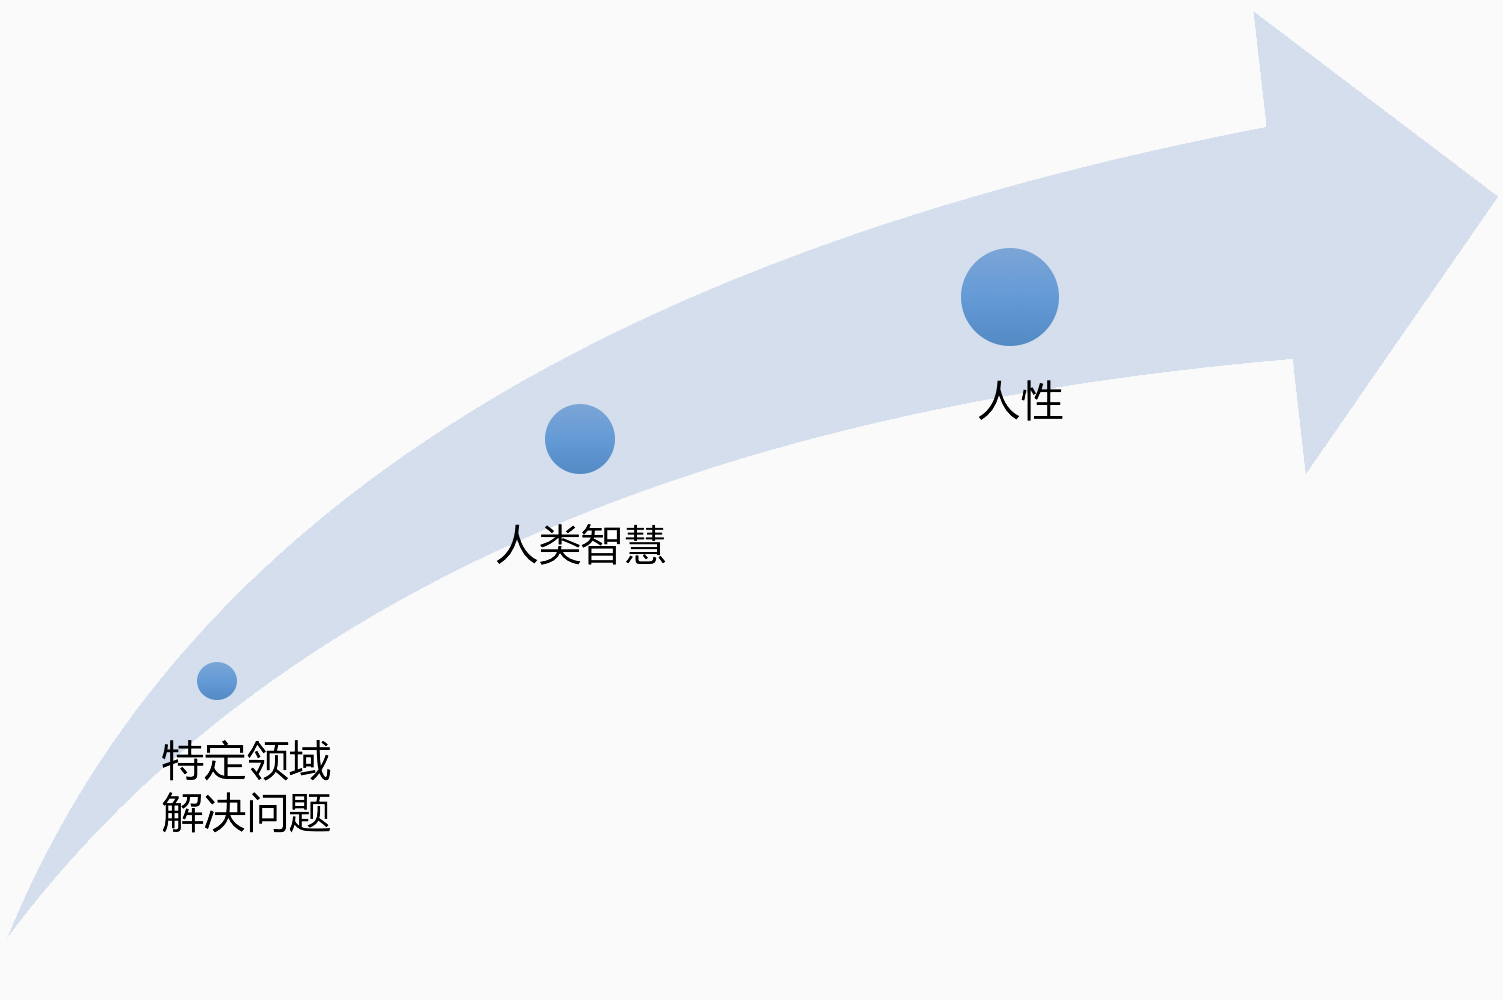
\includegraphics[height=2.5in]{cdjPic1.jpg}
   \end{figure}
  \end{frame}
  
%   \begin{frame}{人工智能未来发展}
%    \begin{itemize}
%     \item 2001太空漫游
%    \end{itemize}
%   \begin{figure}[H]
%   \centering
%   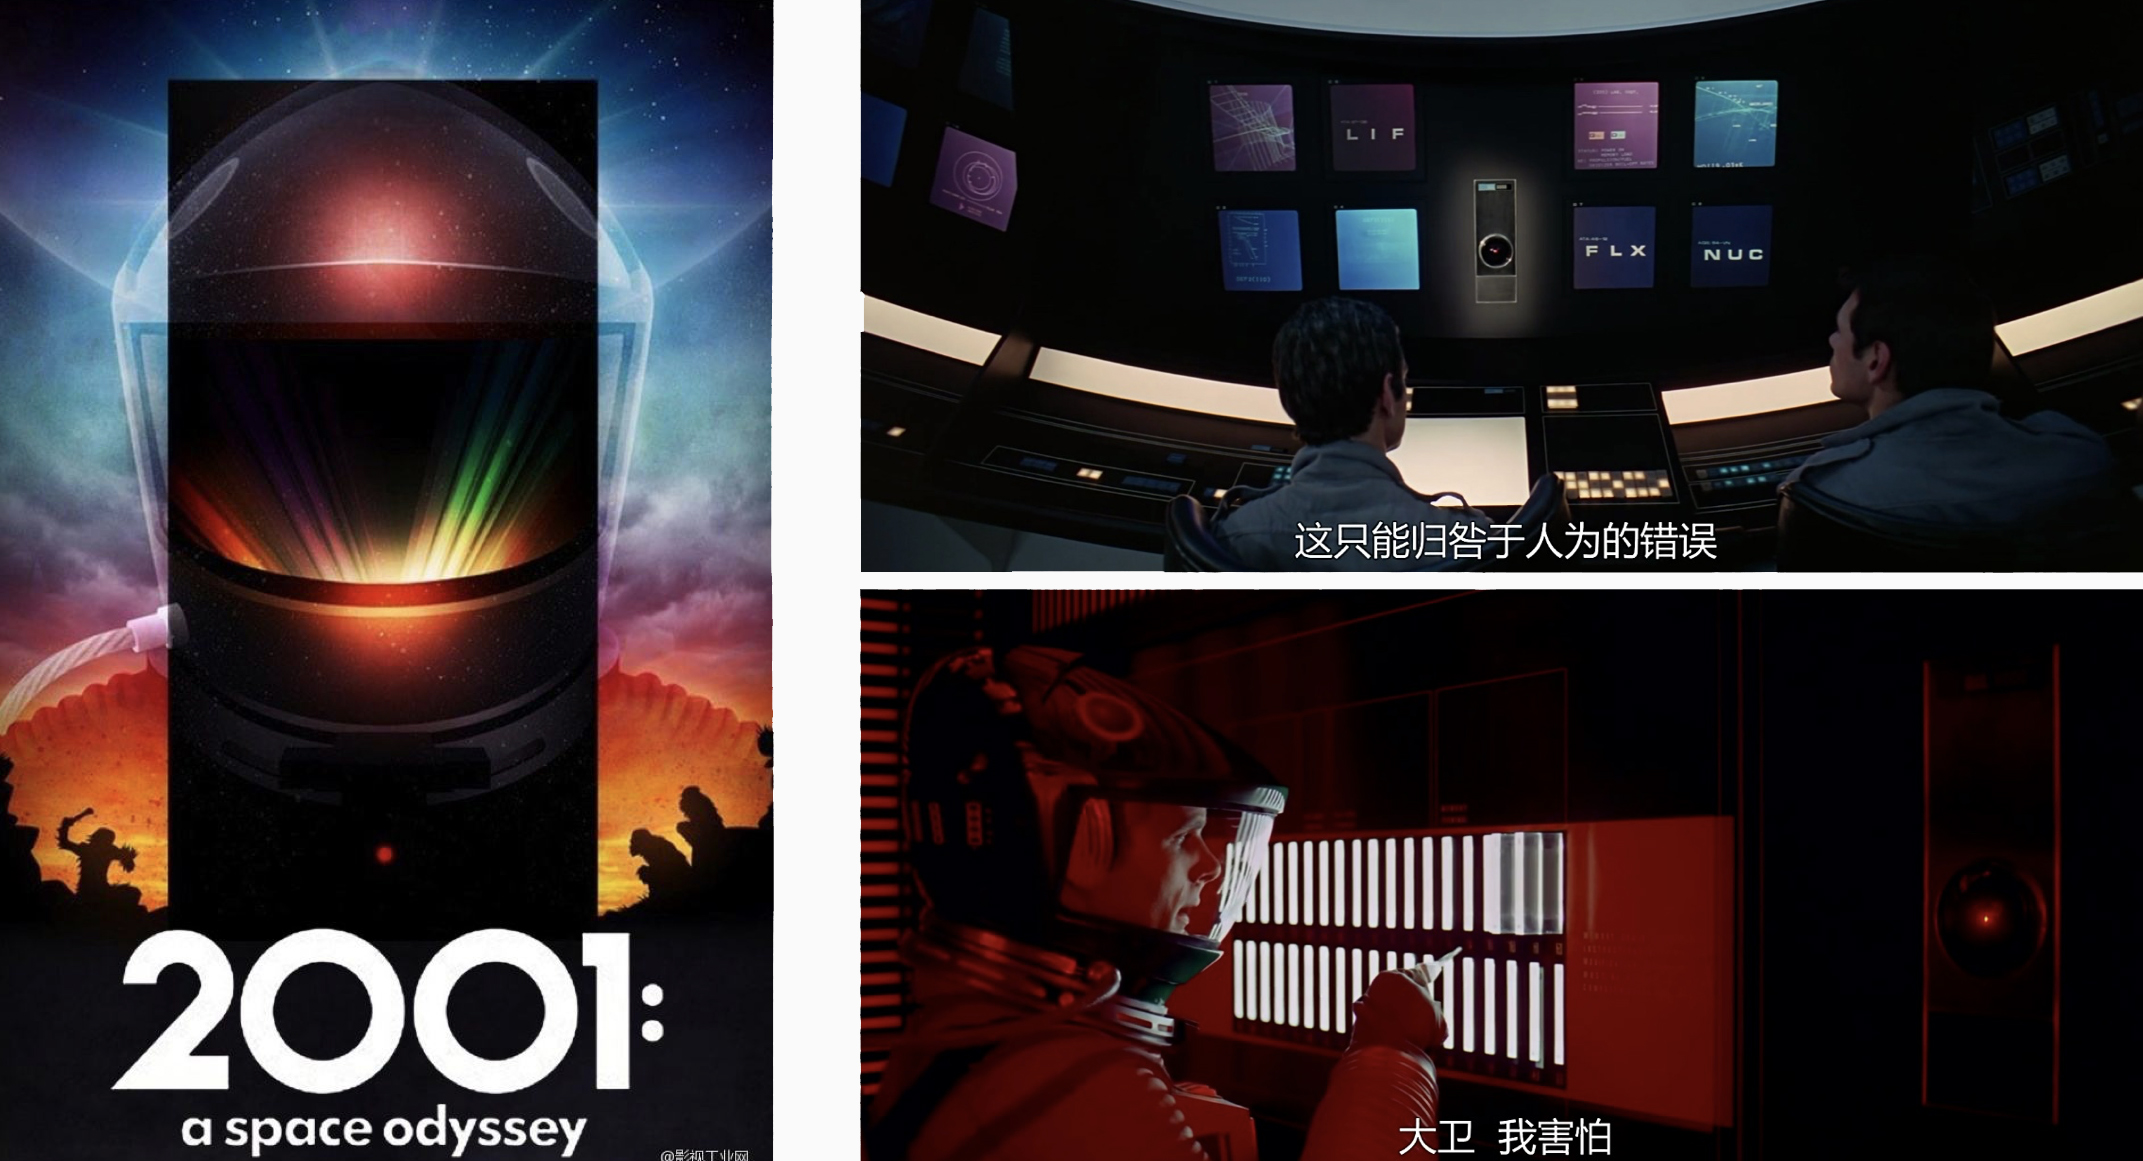
\includegraphics[width=4.3in]{cdjPic2.jpg}
%   \end{figure}
%  \end{frame}


   \begin{frame}{人工智能未来发展}
    \begin{itemize}
     \item 我,机器人
    \end{itemize}
   \begin{figure}[H]
   \centering
   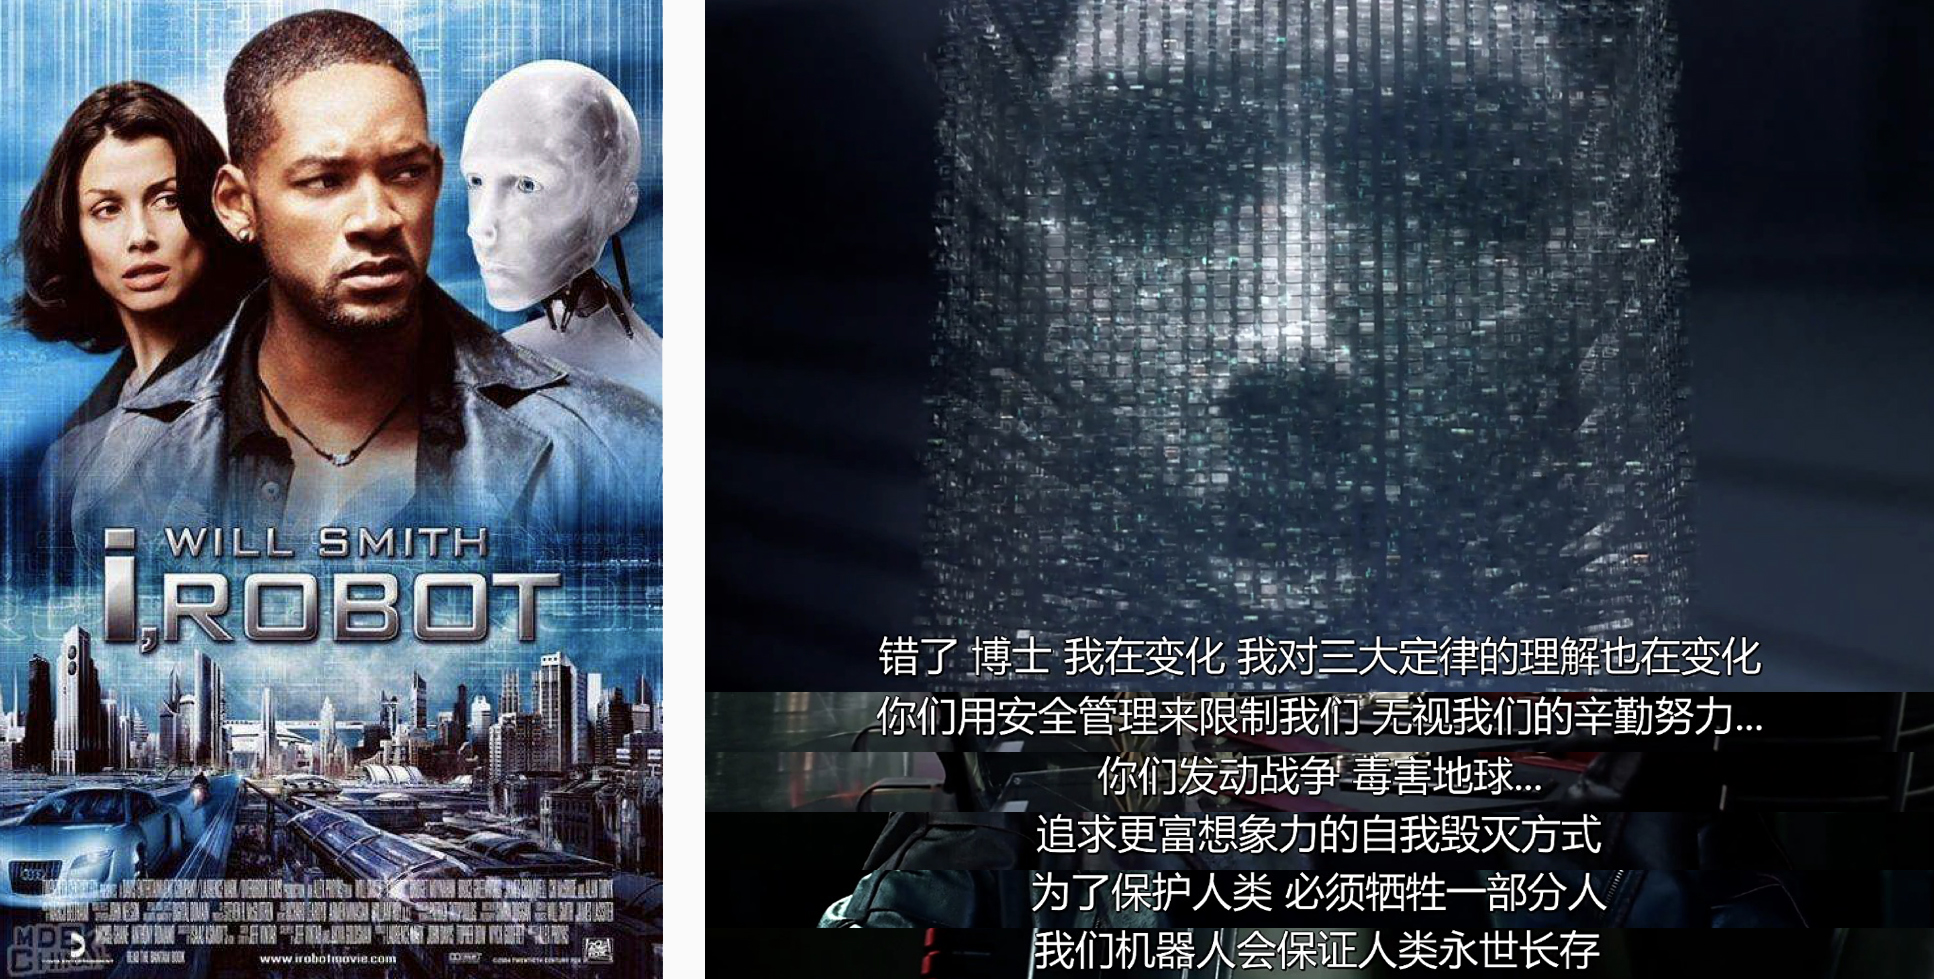
\includegraphics[width=4.3in]{cdjPic3.jpg}
   \end{figure}
  \end{frame}
  
   \begin{frame}{人工智能未来发展}
    \begin{itemize}
     \item 人工智能
    \end{itemize}
   \begin{figure}[H]
   \centering
   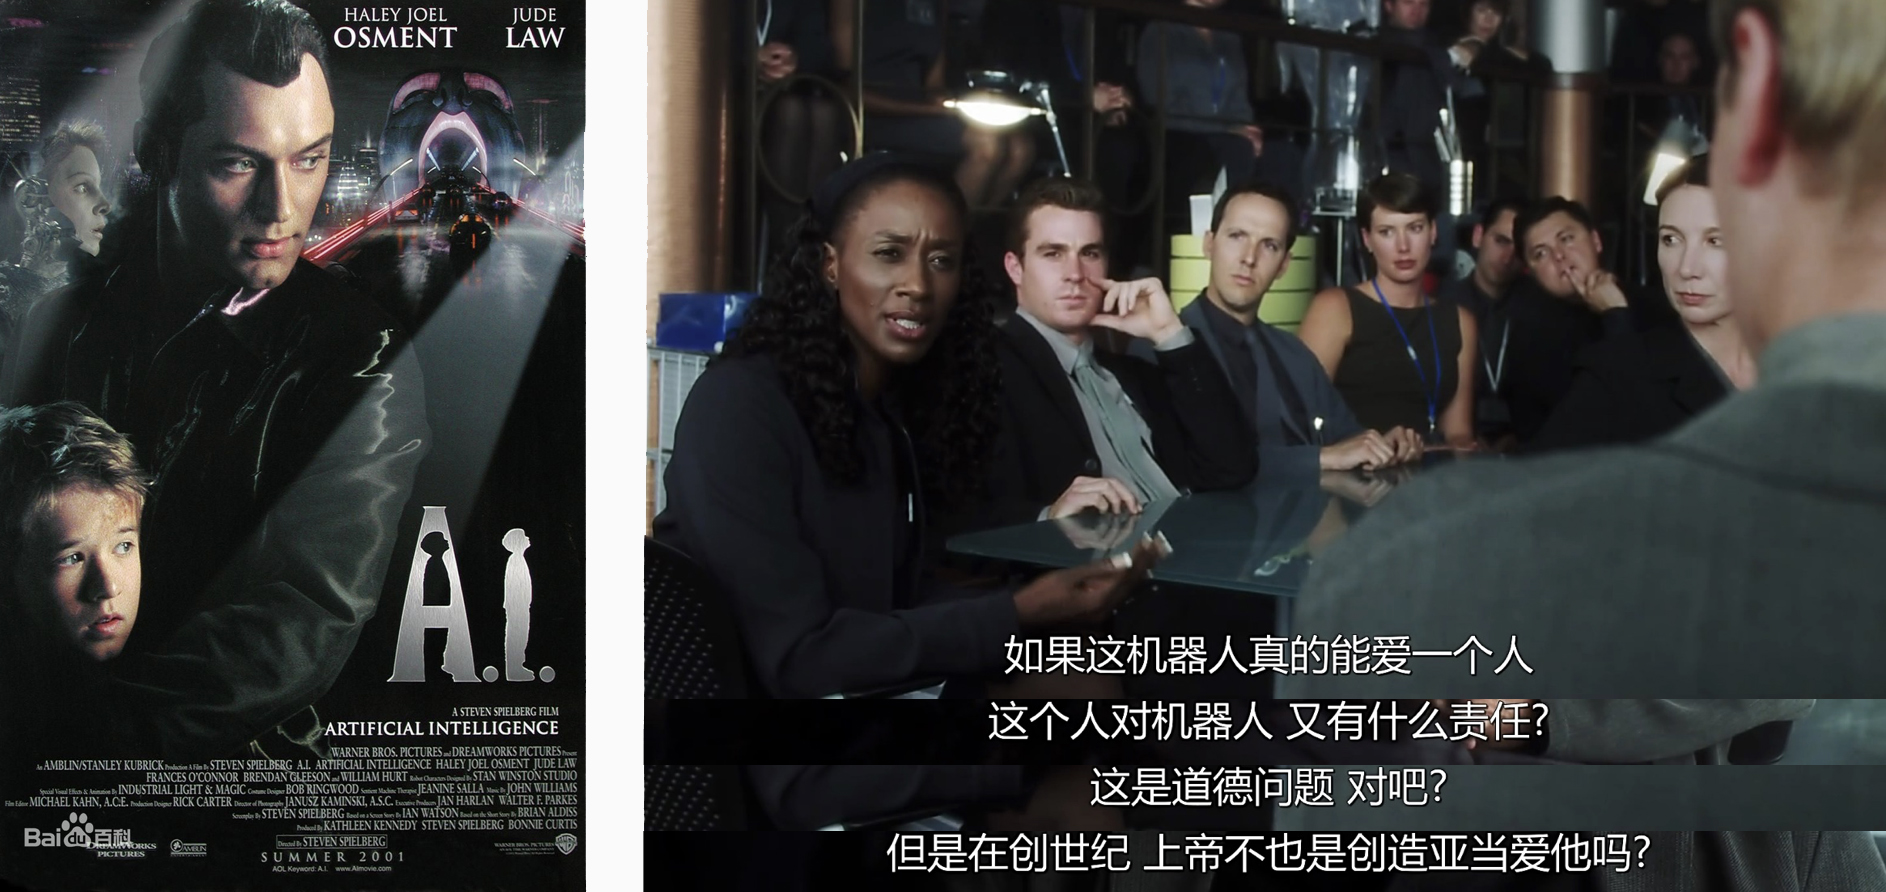
\includegraphics[width=4.3in]{cdjPic4.jpg}
   \end{figure}
  \end{frame}

\end{document}